% !TEX TS-program = LuaLaTeX
% Gemini theme
% https://github.com/anishathalye/gemini

\documentclass[final]{beamer}

% ====================
% Packages
% ====================

%\usepackage[T1]{fontenc}
\usepackage{lmodern}
\usepackage[size=custom,width=106.7,height=80.0,scale=0.85]{beamerposter}% max=135x76
\usetheme{gemini}
\usecolortheme{gemini}
\usepackage{graphicx}
\usepackage{amsmath}
\usepackage{amsfonts,amssymb,latexsym,amscd}
\usepackage[numbers]{natbib}
\usepackage{amsmath}
\usepackage{booktabs}
\usepackage{tikz}
\usepackage{pgfplots}
\usepackage{comment}
\usepackage{scalefnt}
\usepackage{isomath}
\usepackage{subfig}
\usepackage{bm}
\usepackage{multirow}
\usepackage{microtype}
\usepackage{tikz}

\usetikzlibrary{calc,patterns,decorations.pathmorphing,decorations.markings,decorations.pathreplacing}
\usetikzlibrary{shapes,fit}
\usetikzlibrary{positioning}
\usetikzlibrary{decorations.text}
\newcommand\independent{\protect\mathpalette{\protect\independenT}{\perp}}
\def\independenT#1#2{\mathrel{\rlap{$#1#2$}\mkern2mu{#1#2}}}
\newcommand*{\og}{\textcolor{orange}}
\usepackage{listings}
\def\listingsfont{\ttfamily}

\graphicspath{{./Figures/}}
\newcommand{\indep}{\rotatebox[origin=c]{90}{$\models$}}


%%%%%%%%%
%Beambox
%%%%%%%%%
%\setbeamertemplate{blocks}[rounded][shadow=true]
\definecolor{cl_postit}{RGB}{255,255,136}
\setbeamercolor{postit}{fg=black,bg=cl_postit}
\newcommand{\source}[1]{\begin{textblock*}{8cm}(7.95cm,7.7cm)
    \begin{beamercolorbox}[ht=0.5cm,right]{framesource}
        \usebeamerfont{framesource}\usebeamercolor[fg]{framesource} [{#1}]
    \end{beamercolorbox}
\end{textblock*}}
% ====================
% Lengths
% ====================

% If you have N columns, choose \sepwidth and \colwidth such that
% (N+1)*\sepwidth + N*\colwidth = \paperwidth
\newlength{\sepwidth}
\newlength{\colwidth}
\setlength{\sepwidth}{0.025\paperwidth}
\setlength{\colwidth}{0.3\paperwidth}

\newcommand{\separatorcolumn}{\begin{column}{\sepwidth}\end{column}}

  
% ====================
% Title
% ====================

\title{Implementation of probabilistic Softmax for BNNs}
\logoleft{%
%
\includegraphics[width=0.06\paperwidth]{Figures/Polytechnique_logo.pdf}
}
\logoright{%
}
\author{David Wardan, Khalil Sabri, \,and\, Miquel Florensa  -- Polytechnique Montr\'{e}al, Canada}

\institute[shortinst]{}

%% ====================
%% Footer (optional)
%% ====================
%
\footercontent{
%  \href{https://www.example.com}{https://www.example.com} \hfill
  IFT6269 Project Poster 2024 } 
%  \href{mailto:alyssa.p.hacker@example.com}{alyssa.p.hacker@example.com}}


% ====================
% Body
% ====================

\begin{document}
\begin{frame}[t]

\begin{columns}
%%%%%%%%%%
%%% Column 1
%%%%%%%%%%
\begin{column}[T]{.31\textwidth}

{\Large COLUMN 1 (TAGI)}


\end{column}
%%%%%%%%%%
%%% Column 2
%%%%%%%%%%
\begin{column}[T]{.31\textwidth}

{\Large COLUMN 2 (Remax)}


\end{column}
%%%%%%%%%%
%%% Column 3
%%%%%%%%%%
\begin{column}[T]{.31\textwidth}



%% cuTAGI
\begin{block}{py/cuTAGI -- Open-source Bayesian deep-learning framework}\vspace{0pt}\centering


\begin{columns}
\begin{column}{.35\textwidth}\centering\bigskip


\bigskip


\medskip



\includegraphics[width=115mm]{Figures/cupyTAGI.pdf}\\[20pt]


{\texttt{github\!.\!com/lhnguyen102/\!cuTAGI}}\\[20pt]
%{\LARGE\texttt{tagiml.com}}\\[20pt]
{\Large\texttt{\alert{ pip install pytagi}}}
\end{column}
%\begin{column}{.22\textwidth}\centering\vspace{-25pt}
%\includegraphics[width=120mm]{Figures/cutagi_example.pdf}
%\end{column}
\begin{column}{.6\textwidth}
\begin{itemize}
\item \alert{\bf Performance-Oriented Kernels} written in C++/CUDA from scratch, with pybind11 for a seamless integration. It allows running on CPU \& CUDA devices through a Python API.
\item \alert{\bf Broad Architecture Support} of the basic DNN layer including \emph{\color{darkblue}\bf Linear}, \emph{\color{cyan}\bf CNNs}, \emph{\color{blue}\bf Transposed CNNs}, \emph{\color{magenta}\bf LSTM}, \emph{\color{orange}\bf Average pooling}, \emph{\color{teal}\bf Batch} and \emph{\color{violet}\bf Layer normalization}, enabling the building of mainstream architectures such as \emph{Autoencoders}, \emph{Transformers}, \emph{Diffusion Models}, and \emph{GANs}.
\item \alert{\bf Model Building and Execution} currently supports sequential model building, with plans to introduce Eager Execution
\item \alert{\bf Open Platform} providing access to its entire codebase. 
\end{itemize}


\end{column}
\end{columns}
\end{block}%\bigskip
\vspace{-5mm}


 
%% cuTAGI
\begin{block}{TAGI-related references}\vspace{10pt}


\begin{columns}
\begin{column}{.15\textwidth}\centering

\includegraphics[width=30mm]{Figures/cuTAGI_refs_QR.pdf}\\[5pt]

\includegraphics[width=20mm]{Figures/IJF.jpg}\\[5pt]
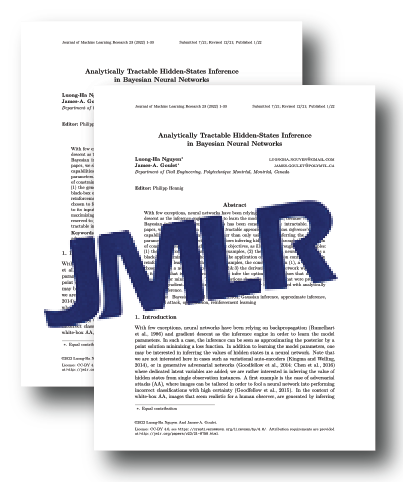
\includegraphics[width=22mm]{Figures/TAGI_AA_JMLR_2.png}
\end{column}\hspace{-20mm}


\begin{column}{.79\textwidth}
\begin{itemize}
\item \emph{\alert{\bf Coupling LSTM Neural Networks and SSM through Analytically Tractable Inference}},\\(Vuong, Nguyen \& Goulet, International Journal of Forecasting, 2024)
\item \emph{Analytically tractable hidden-states inference in Bayesian neural networks}\\ (Nguyen and Goulet. Journal-to-conference track, ICLR 2024)
\item \emph{Analytically tractable heteroscedastic uncertainty quantification in Bayesian neural networks for regression tasks}\\ (Deka, Nguyen \& Goulet. Neurocomputing, 2024)
\item \emph{Tractable approximate Gaussian inference for Bayesian neural networks}\\ (Goulet, Nguyen, \& Amiri, JMLR, 2021)
%\item \emph{Analytically tractable inference in deep neural networks}\\ (Nguyen and Goulet. 2021)
%\item \emph{Analytically tractable Bayesian deep Q-Learning} (Nguyen and Goulet. 2021)
\end{itemize}
\end{column}
\end{columns}
\end{block}




\end{column}
%%%%%%%%%%%
%%%% Column 4
%%%%%%%%%%%
%\begin{column}[T]{.25\textwidth}
%\end{column}
\end{columns}
\end{frame}
\end{document}
